\documentclass[12pt]{article}


\usepackage[spanish]{babel}
\selectlanguage{spanish}
\usepackage[utf8]{inputenc}
\usepackage{graphicx}


\title{Iniciando con Fortran}
\author{Valenzuela Coronado Paulina}
\date{Licenciatura en Física}


\begin{document}
\maketitle

\section{Actividad 3}
Esta actividad se baso en realizar una serie de programas que solucionaban problemas matemáticos de una forma más sencilla y rápida para el usuario.
Estos programas se realizaron usando el lenguaje Fortran.

\section{A continuacion se presentan distintos códigos con los que trabajamos:}

\begin{itemize}
\item {\tt Área de un circulo} 
\begin{figure}[h]
\centering
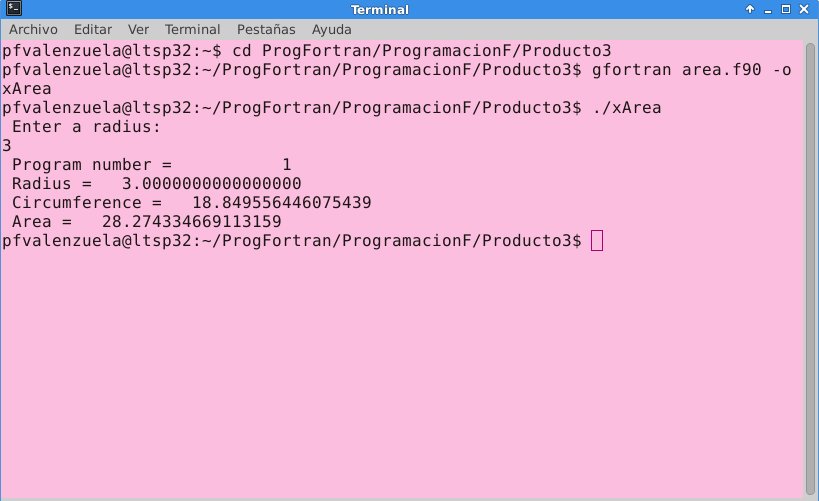
\includegraphics[scale=0.5]{area.png}
\end{figure}
\begin{verbatim}

! Area . f90 : Calculates the area of a circle, sample program
! ---------------------------------
 Program areadelcirculo ! Begin main program
  Implicit None ! Declare all variables
   Real *8 :: radius , circum , area ! Declare Reals
   Real *8 :: PI = 4.0 * atan(1.0) ! Declare , assign Real
  Integer :: model_n = 1 ! Declare , assign Ints
   print * , 'Enter a radius:' ! Talk to user
   read * , radius ! Read into radius
  circum = 2.00 * PI * radius ! Calc circumference
  area = radius * radius * PI ! Calc area
  print * , 'Program number =' , model_n ! Print program number
  print * , 'Radius =' , radius ! Print radius
  print * , 'Circumference =' , circum ! Print circumference
  print * , 'Area =' , area ! Print area
 End Program areadelcirculo ! End main program code
 \end{verbatim}

\item {\tt Función}
\begin{figure}[h]
\centering
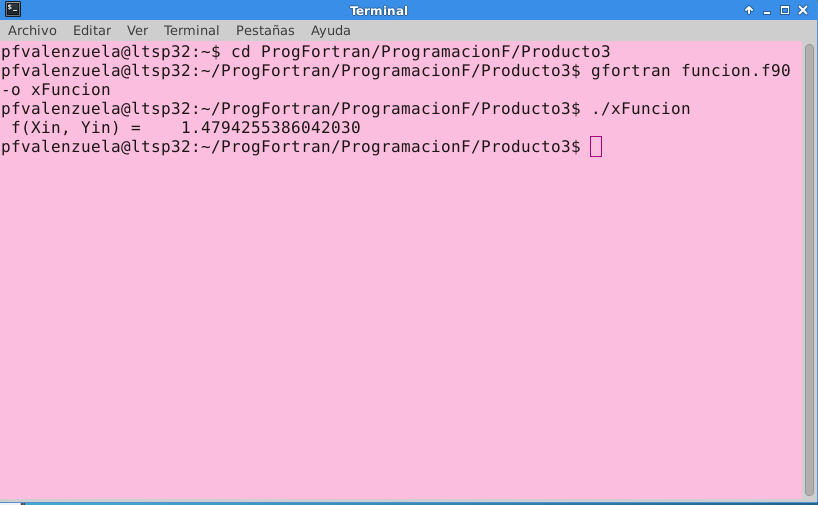
\includegraphics[scale=0.5]{funcion.png}
\end{figure}
\begin{verbatim}
 
 ! Function . f90 : Program calls a simple function
 !--------------------------------------
 Real *8 Function f (x,y)
   Implicit None
   Real *8 :: x, y
   f = 1.0 + sin (x*y )
 End Function f
 !
 Program Main
  Implicit None 
  Real *8 :: Xin =0.25 , Yin =2. , c , f ! declarations ( also f)
  c = f ( Xin , Yin )
  write ( * , * ) 'f(Xin, Yin) = ' , c
 End Program Main 
 \end{verbatim}
 
\item {\tt Math } 
\begin{figure}[h]
\centering
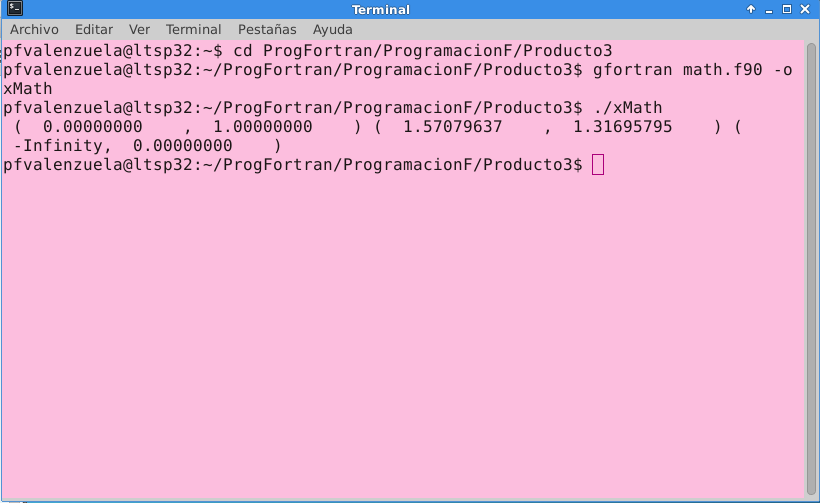
\includegraphics[scale=0.5]{math.png}
\end{figure}
\begin{verbatim}
 ! Math . f90 : demo some Fortran math functions
 ! ----------------------------------
 Program Math! Begin main program

   Complex *8 :: x=- 1.0 , y=2.0, z=0 ! Declare variables x, y, z
  x = sqrt (x)  
  y = asin (y) ! Call the asine function
  z = log (z) ! Call the log function
  print * , x, y, z ! Print x, y, z
 End Program Math ! End main program 
\end{verbatim}
 
 \item {\tt Precisión}
 \begin{figure}[h]
\centering
\includegraphics[scale=0.5]{presicion.png}
\end{figure}
 
 \begin{verbatim}
 ! Limits . f90 : Determines machine precision
 ! ----------------------------------
 Program Limits
   Implicit None
   Integer :: i , n
   Real *4 :: epsilon_m , one
   n=60 ! Establish the number of iterations
   ! Set initial values :
   epsilon_m = 1.0
  one = 1.0
  ! Within a DO−LOOP, calculate each step and print .
  ! This loop will execute 60 times in a row as i is
  ! incremented from 1 to n ( since n = 60) :

  do i = 1, n , 1 ! Begin the do−loop
    epsilon_m = epsilon_m / 2.0 ! Reduce epsilon m
    one = 1.0 + epsilon_m ! Re−calculate one
    print * , i , one , epsilon_m ! Print values so far
  end do ! End loop when i>n
 End Program Limits 
\end{verbatim}
 
 \item {\tt Subroutine}
 \begin{figure}[h]
\centering
 \includegraphics[scale=0.5]{subrutina.png}
\end{figure}
\begin{verbatim}
 Subroutine g(x, y , ans1 , ans2)
  Implicit None
  Real (8) :: x , y , ans1 , ans2 ! Declare variables
  ans1 = sin (x*y) + 1. ! Use sine intrinsic funcion
  ans2 = ans1**2
End Subroutine g
!

Program Main 
  Implicit None
  Real *8 :: Xin = 0.25 , Yin = 2.0 , Goutl , Gout2
  call g( Xin , Yin , Goutl , Gout2 ) ! Call the subr g
  write ( * , * ) 'The answers are: ' , Goutl , Gout2

End Program Main 
 \end{verbatim}
 
  \item {\tt Volumen}
  \begin{figure}[h]
\centering
\includegraphics[scale=0.5]{volumen.png}
\end{figure}
  \begin{verbatim}
  ! Area . f90 : Calculates the area of a circle, sample program
 ! ------------------------------------------
 Program volumendelaesfera! Begin main program
  Implicit None ! Declare all variables
   Real *8 :: radius , height , newradius, volume ! Declare Reals
   Real *8 :: PI = 4.0 * atan(1.0) ! Declare , assign Real
  Integer :: model_n = 1 ! Declare , assign Ints
   print * , 'Enter a Radius:' ! Talk to user
   read * , radius ! Read into radius
   print * , 'Enter a Height:' ! Talk to user
   read * , height ! Take the value of h
  newradius = 3.00 * radius - height 
  volume = 0.333 * PI * height * height * newradius ! Calc Volume
  print * , 'Program number =' , model_n ! Print program number
  print * , 'Radius =' , radius ! Print radius
  print * , 'Height =' , height ! Print height
  print * , 'Volume =' , volume ! Print volume
 End Program volumendelaesfera ! End main program code
  
  \end{verbatim}
 
 
\end{itemize}



\end{document}